\section{Implementaiton}
\label{imp}

In this paper we are going to suggest a solution for porting part of xv6-riscv \cite{xv6} to a paravirtalization setup. It is not within scope of this report to do a complete port but rather illustrate trough some of the system components how it could be implemented with a compatible hypervisor. The idea here is to replace hardware specific calls to io memory with a syscall that calls on our hypervisor to-do the required function. This call is also called a hypercall but in essence it’s just another exception we send to the program running a level over us. 

The system component we are going to look specifically at is the console/shell of the xv6 kernel. Currently in the latest iteration of the xc6-riscv \cite{xv6} code base (as of writing this paper). The console uses UART (Universal Asynchronous Receiver/Transmitter) driver for the 16550 UART. This is originally based on a chip by National Semiconductor but since the chip and interface got so well adopted it is generally used in virtualization applications. Since xv6 by default support qemu we can assume that qemus console output interface is 16550 UART based on the guest side. Our hypothetical hypervisor than needs to support this interface and have a driver for it if we wish to continue and use qemu for console output.


\begin{figure}[htbp]
    \centering
    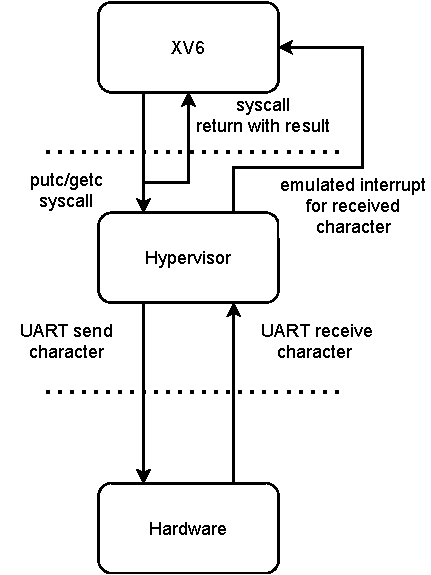
\includegraphics[width=0.5\textwidth]{Images/tdt09_uart_hypervisor.drawio.pdf}
    \caption{High level visualization of implementaiton}
    \label{fig:uart-hype-hardware}
\end{figure}

\newpage
Figure \ref{fig:uart-hype-hardware} shows the uart implementaiton on a higher level and what we expect the hypervisor and XV6 todo to get a character out on the screen. In practice we can think of the uart driver we see in xv6 now being moved to our hypervisor with a syscall handler wrapper that calls it. In the case of recived characters from the uart hardware in another word user input, the hypervisor can then emulate a interrupt in its own interrupt handler code for the uart to send the recived characters to xv6.

Currently in \textbf{kernel/console.c} and  \textbf{kernel/uart.c} we have the current use of the uart driver:

\textbf{kernel/console.c line 34}
\begin{minted}{c}
//
// send one character to the uart.
// called by printf, and to echo input characters,
// but not from write().
//
void consputc(int c)
{
  if(c == BACKSPACE){
    // if the user typed backspace, overwrite with a space.
    uartputc_sync('\b'); uartputc_sync(' '); uartputc_sync('\b');
  } else {
    uartputc_sync(c);
  }
}
\end{minted}

\textbf{kernel/console.c line 59}
\begin{minted}{c}
//
// user write()s to the console go here.
//
int consolewrite(int user_src, uint64 src, int n)
{
  int i;

  for(i = 0; i < n; i++){
    char c;
    if(either_copyin(&c, user_src, src+i, 1) == -1)
      break;
    uartputc(c);
  }

  return i;
}
\end{minted}

\textbf{kernel/console.c line 182}
\begin{minted}{c}
void consoleinit(void)
{
  initlock(&cons.lock, "cons");

  uartinit();

  // connect read and write system calls
  // to consoleread and consolewrite.
  devsw[CONSOLE].read = consoleread;
  devsw[CONSOLE].write = consolewrite;
}
\end{minted}

\textbf{kernel/uart.c line 180}
\begin{minted}{c}
// handle a uart interrupt, raised because input has
// arrived, or the uart is ready for more output, or
// both. called from trap.c.
void uartintr(void)
{
  // read and process incoming characters.
  while(1){
    int c = uartgetc();
    if(c == -1)
      break;
    consoleintr(c);
  }

  // send buffered characters.
  acquire(&uart_tx_lock);
  uartstart();
  release(&uart_tx_lock);
}
\end{minted}

\newpage
\subsection{Console Write}
\label{imp:console-write}

Based on what we can see from above we have two different functions that needs to be replaced when it comes to uart write:
\begin{minted}{c}
    uartputc();
    uartputc_sync();
\end{minted}

The difference between \textbf{uartputc()} and \textbf{uartputc\_sync()} is that sync does not use interrupts and therefore can be used to print characters to the screen in case of a kernel panic. Since we are going to replace this with a syscall we can just use the same function for this.

Then a suggested replacement implementation for the uartputc function could be these two functions.

\begin{minted}{c}
// Generic syscall wrapper for Riscv64
static inline long syscall(long n, long _a0, long _a1, long _a2, 
                            long _a3, long _a4, long _a5){
  register long a0 asm("a0") = _a0;
  register long a1 asm("a1") = _a1;
  register long a2 asm("a2") = _a2;
  register long a3 asm("a3") = _a3;
  register long a4 asm("a4") = _a4;
  register long a5 asm("a5") = _a5;
  register long syscall_id asm("a7") = n;

  asm volatile ("scall"
		: "+r"(a0) : "r"(a1), "r"(a2), "r"(a3), 
        "r"(a4), "r"(a5), "r"(syscall_id));

  return a0;
}

#define SYSCALL_PUTC 10

void hypercall_putc(char c){

    syscall(SYSCALL_PUTC, c, 0, 0, 0, 0, 0);

}
\end{minted}

The code above assumes that the hypervisor has a syscall which is identified with 10. There is no reason to why 10 specifically is chosen as a number and this can be changed arbitrarily. The character is supplied directly in one of the argument registers. It takes the same input as uartputc but formats it into a syscall that is sent to the hypervisor instead of interacting directly with the hardware. Since our syscall function also returns a value, we could also do some checking if for some reason our hypercall failed. Though we have opted to not do this in this scenario.  

\newpage
\subsection{Console Read}
\label{imp:console-read}

When it comes to read we need the hypervisor to call our interrupt handler for for our console:

\begin{minted}{c}
    consoleintr();
\end{minted}

This can be done by changing the call to \textbf{uartintr()} which we find at \textbf{kernel/trap.c line 189} to \textbf{consoleintr()}
\begin{minted}{c}
    if(irq == UART0_IRQ){
      uartintr();
    } else if(irq == VIRTIO0_IRQ){
      virtio_disk_intr();
    } else if(irq){
      printf("unexpected interrupt irq=%d\n", irq);
    }
\end{minted}

We are now though relining on the hypervisor to generate the necessary interrupt to XV6  and pass the character through a shared memory location or one of the registers

